% Source: https://www.dropbox.com/sh/rl0yyth9g06psva/AADB0Cj4isIX5DAyrspqj8mFa
% File: "CS305 activity 12 binary search trees.pdf"
% Access: 05-18-2022

% comment out for student version
%\ifdefined\Student\relax\else\def\Teacher{}\fi

\documentclass[12pt]{article}

\title{Activity \#8: Binary Search Trees}
\author{Tammy VanDeGrift}
\newcommand{\activityeditor}{Preston Carman}
\newcommand{\activitysource}{\url{https://www.dropbox.com/sh/rl0yyth9g06psva/AADB0Cj4isIX5DAyrspqj8mFa}}
\date{Spring 2022}

\input{../cspogil.sty}

% Included for drawing trees
\usepackage{tikz-qtree}
\tikzset{every tree node/.style={minimum width=2em,draw,circle},
         blank/.style={draw=none},
         edge from parent/.style=
         {draw,edge from parent path={(\tikzparentnode) -- (\tikzchildnode)}},
         level distance=1.25cm}

\begin{document}

\begin{center}
  \Large Activity \#8: Binary Search Trees \\[5pt]
  \large Recorder's Report\\[20pt]
  \normalsize
  \begin{tabular}{lrp{0.1in}lr}
    Manager:  & \ans{} &  & Reader: & \ans{}                       \\[15pt]
    Recorder: & \ans{} &  & Driver: & \ans{}                       \\[15pt]
    Date:     & \ans{} &  & Score:  & Satisfactory \hspace{10pt} /
    \hspace{10pt} Not Satisfactory
  \end{tabular}
\end{center}
\par\vskip 15pt

Record your team's answers to the key questions (marked with
\raisebox{-.3\height}{\includegraphics[width=0.5in]{../figures/key.png}})
below.
\begin{enumerate}[label=(\alph*)]
  \itemsep 1.25in
  \item Model 2, Question \#7, 8
  \item Model 2, Question \#10
  \item Model 2, Question \#13
  \item Model 3, Question \#17
\end{enumerate}

\newpage
\maketitle

Binary search trees allow binary search for fast lookup, addition, and removal of data items, and can be used to implement dynamic sets and lookup tables.
Since the nodes in a BST are laid out in such a way that each comparison skips about half of the remaining tree, the lookup performance is proportional to that of binary logarithm.
%\rolenames

\guide{
  \item Explain a binary search tree (BST)
  \item Knowledge of the rules for a BST
}{
  \item Write code that adds and accesses a BST
}{
  No additional notes.
}

\newpage
\model{BST Basics}

A \textbf{BINARY SEARCH} tree is a binary tree in which the data (keys) are stored in order such that all nodes to the right of node N have keys bigger than N and all nodes to the left of node N have keys smaller than N.
\par\vskip 10pt

BSTs give us a good data structure to implement the dictionary ADT (insert, find, delete, create, print).
\par\vskip 10pt

Here is a simple BST where the keys are ints:
\par\vskip 10pt

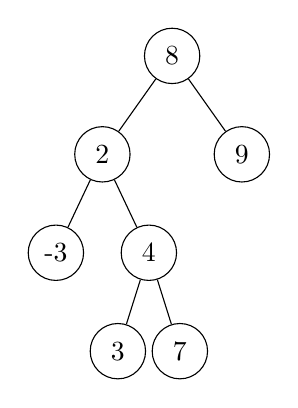
\begin{tikzpicture}
    \Tree
    [.8
    [.2
    -3
    [.4
    3
    7
    ]
    ]
    9
    ]
\end{tikzpicture}

\begin{itemize}
    \item Choose any node in the tree.
    \item Its left subtree descendants are less than the node's value.
    \item Its right subtree descendants are greater than the node's value.
\end{itemize}

\Q Is this a valid binary search tree? \ans[.5in]{} yes \ans[.5in]{X} no

If no, explain why.

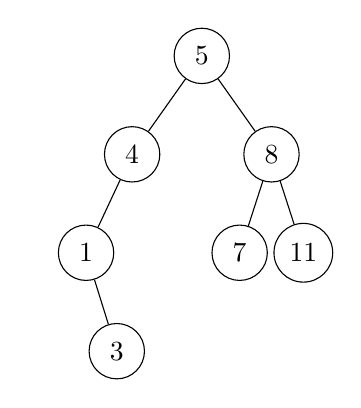
\begin{tikzpicture}
    \Tree
    [.5
            [.4
                    [.1
                        \edge[blank]; \node[blank]{};
                        3
                    ]
                \edge[blank]; \node[blank]{};
            ]
            [.8
                7
                11
            ]
    ]
\end{tikzpicture}

\newpage
\Q Is this a valid binary search tree? \ans[.5in]{X} yes \ans[.5in]{} no

If no, explain why.

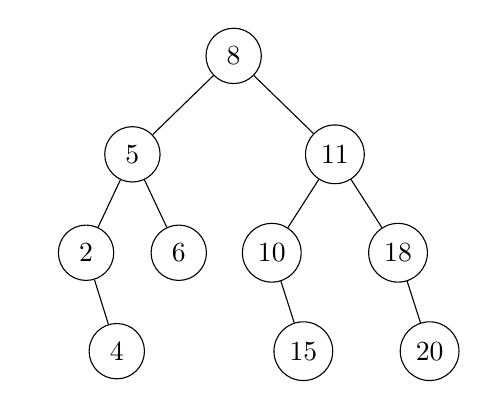
\begin{tikzpicture}
    \Tree
    [.8
            [.5
                    [.2
                        \edge[blank]; \node[blank]{};
                        4
                    ]
                6
            ]
            [.11
                    [.10
                        \edge[blank]; \node[blank]{};
                        15
                    ]
                    [.18
                        \edge[blank]; \node[blank]{};
                        20
                    ]
            ]
    ]
\end{tikzpicture}

\Q Is this a valid binary search tree? \ans[.5in]{X} yes \ans[.5in]{} no

If no, explain why.

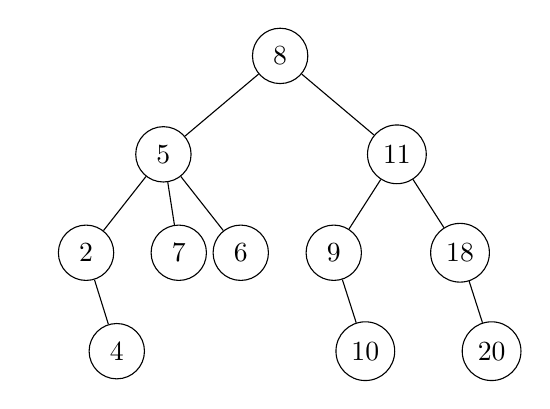
\begin{tikzpicture}
    \Tree
    [.8
            [.5
                    [.2
                        \edge[blank]; \node[blank]{};
                        4
                    ]
                7
                6
            ]
            [.11
                    [.9
                        \edge[blank]; \node[blank]{};
                        10
                    ]
                    [.18
                        \edge[blank]; \node[blank]{};
                        20
                    ]
            ]
    ]
\end{tikzpicture}

\textbf{Inserting new nodes}

How do we insert new nodes into a BST?


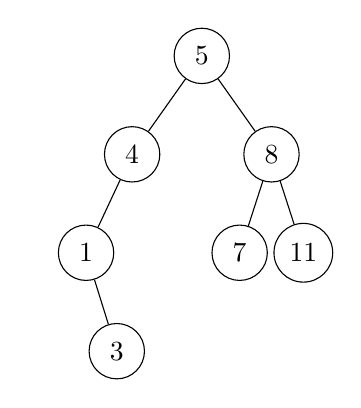
\begin{tikzpicture}
    \Tree
    [.5
            [.4
                    [.1
                        \edge[blank]; \node[blank]{};
                        3
                    ]
                \edge[blank]; \node[blank]{};
            ]
            [.8
                7
                11
            ]
    ]
\end{tikzpicture}


\Q Suppose we want to insert the value 6. Where does it go?

\Q Now, we want to insert 0. Where does it go?

\Q Now, we want to insert 9. Where does it go?

\newpage
Inserting into a BST is quite simple. Insertions happen at the leaves.
Here is an iterative version:

\footnotesize
\begin{cpplst}
/* insert
 * inserts data item d into tree; note that this is a BST so it is ordered
 */
void insert(TreeData d, TreeNode **tptr) {
    // create new node for data
    TreeNode *toInsert = newTreeNode(d);
    TreeNode *curr = *tptr;
    if (curr == NULL) {
        *tptr = toInsert; // make this the tree
        return;
    }
    // check value of t to see if new node should be to the right or left of curr
    while (curr != NULL) {
        if (d < curr->value) { // goes to left
            if (curr->left == NULL) {
                curr->left = toInsert;
                return;
            }
            // keep going left
            curr = curr->left;
        } else { // goes to right
            if (curr->right == NULL) {
                curr->right = toInsert;
                return;
            }
            // keep going right
            curr = curr->right;
        }
    }
}
/* newTreeNode
 * helper function, creates a new tree node with value d
 * returns the address of the new node
 */
TreeNode *newTreeNode(TreeData d) {
    TreeNode *toReturn = (TreeNode *)malloc(sizeof(TreeNode));
    toReturn->value = d;
    toReturn->left = NULL;
    toReturn->right = NULL;
    return toReturn;
}
\end{cpplst}

\normalsize
Here is a recursive version to insert an item:

\footnotesize
\begin{cpplst}
/* insertR (this function is written recursively)
 * inserts data item d into tree; note that this is a BST so it is ordered
 */
void insertR(TreeData d, TreeNode **tptr) {
    if (*tptr == NULL) {
        *tptr = newTreeNode(d);
    } else if (d < (*tptr)->value) {
        insertR(d, &(*tptr)->left);
    } else {
        insertR(d, &(*tptr)->right);
    }
}
\end{cpplst}
\normalsize

\newpage

\model{Binary Trees}

A tree is a fundamental data structure in computing.
We generally draw trees with the root node at the top of the tree (upside-down from regular trees you see in nature).
\par\vskip 10pt

\includegraphics[width=.9\textwidth]{figures/trees_example.png}

\textbf{Some more vocabulary about trees:}

\textit{Children} are ordered left to right; a parent could have 0 or more children.

A tree with 0 nodes is an \textit{empty} tree.

\textit{Ancestors} of a node N are the nodes in the path from N to the root of the tree.

\textit{Descendants} of a node N are the set of nodes that can be reached from any downward path from N.

The \textit{height} of the tree is the number of nodes along the longest (deepest) path of the tree.
The height of an empty tree is 0.

The \textit{subtree} at node N is node N with all its descendants.

\Q How could trees be useful for modeling data in computing applications?

\begin{answer}[1in]
\end{answer}

\begin{itemize}
    \item Example: From Java, class hierarchies.
    \item Example: From Coding, recursive function calls (hw 2, mazes).
    \item Example: From Data Compression, Huffman coding.
    \item Example: From Phone Menus, sequence of instructions (press 1 if you want to make a reservation, press 2 if you want to check on a reservation, press 3 if you want to speak to an operator; pressing 1 then asks, press 1 if you are making a reservation within the US, press 2 if you are making a reservation within Canada, etc.)
\end{itemize}
\par\vskip 10pt

A \textbf{BINARY} tree is a tree in which each node has at most two children.
Children are named left child or right child.

Each node contains:

\begin{tabular}{|l|}
    \hline
    Data (key,value) pairs if a dictionary \\ \hline
    Left child                             \\ \hline
    Right child                            \\ \hline
\end{tabular}

\begin{cpplst}
typedef int TreeData; // can change type with primitive or struct type
typedef struct TreeNodeTag TreeNode;

struct TreeNodeTag {
  TreeData value; // value stored in node
  TreeNode * left; // left child
  TreeNode * right; // right child
};
\end{cpplst}


The left child is a pointer to another tree node.
The right child is a pointer to another tree node.
For simplicity, we will store just one data item per node (but this data item could be a struct that contains key, value pairs).
\par\vskip 10pt

Suppose T is a binary tree, where each node has at most two children.

\Q Draw a binary tree with 6 nodes (labeled A, B, C, D, E, F) where there are exactly 3 leaves.


\begin{answer}[1.5in]
\end{answer}


Recall that the height of a tree is the number of nodes of the longest (deepest) path from the root to a leaf node.

\par\vskip 10pt

What is the height of your tree? \ans{}

\par\vskip 10pt


\Q Draw a binary tree with 6 nodes where there is exactly 1 leaf.

\begin{answer}[1.5in]
\end{answer}

What is the height of your tree? \ans{}

\newpage
Assume a binary tree has height H.

\Q What is the maximum \# of leaf nodes in a tree of height H? \ans{}

\Q What is the maximum \# of nodes in a tree of height H? (pack them in) \ans{}

\Q What is the minimum \# of leaf nodes in a tree of height H? \ans{}

\Q What is the minimum \# of nodes in a tree of height H? \ans{}

\par\vskip 10pt

\textit{In general, trees only speed things up if the tree is ``full'', meaning that we have close to the maximum number of nodes in a tree for a given height.
    A long, skinny tree does not outperform a linked list.}
\par\vskip 10pt

Here is a binary tree of arithmetic expressions.


\includegraphics[width=.4\textwidth]{figures/trees_arithmetic_expression.png}

We can traverse the tree in one of three ways:

\begin{itemize}
    \item Preorder: examine node, left subtree, right subtree
    \item Inorder: examine left subtree, node, right subtree
    \item Postorder: examine left subtree, right subtree, node
\end{itemize}

If you get confused about the names, think about \textbf{*when*} the node is examined. First (pre), Second (in), Third (post).

In the example above, here are the orders of these traversals:

\begin{itemize}
    \item Preorder: + x 2 5 4
    \item Inorder: 2 x 5 + 4
    \item Postorder: 2 5 x 4 +
\end{itemize}

Sometimes, the order of traversal does not matter for certain operations.
For example, if you want to know how many nodes are in a tree, the way you traverse the tree does not impact your result.
Any traversal would be fine.
Sometimes, though, order does matter.
If you want to print a tree such that each level of a tree is indented further to the right, you would want to examine the tree in preorder fashion.
If you are evaluating an expression tree, such as the one above, you would want to do this in postorder (get value of children before processing new operator).

Here is the code for inorder traversal. Note that visit is also defined for visiting the node.

\begin{cpplst}

/* inorder
 * visits the nodes inorder (left, current, right) traversal
 */
void inorder(TreeNode * t) {
  if(t != NULL) {
    inorder(t->left);
    visit(t);
    inorder(t->right);
  }
}
\end{cpplst}


\Q Write the code to do preorder traversal:

\begin{cpplst}
void preorder(TreeNode * t) {










}
\end{cpplst}


Suppose a tree has this structure:

\includegraphics[width=.3\textwidth]{figures/trees3.png}

\Q What is the inorder traversal of this tree? \ans{}

\Q What is the preorder traversal of this tree? \ans{}

\newpage
\Q Write the recursive function to return the number of leaves in a tree.
This should be written recursively, since the tree data structure is recursive.
Recall that if t is null, there are no leaves.
If it's right child and left child are both null, t is a leaf, so return 1.
Else, add together the recursive calls to process the left subtree and right subtree.

\begin{cpplst}
int numLeaves(TreeNode * t) {








}
\end{cpplst}

\Q Write a function to count the number of interior nodes with two children.

\begin{answer}[1.5in]
\end{answer}

\Q Assume a binary tree is traversed in-order and preorder.
Here is the output.
What does the tree look like?

Inorder: E F D B A C G H

Preorder: D E F G A B C H

\begin{answer}[2in]
\end{answer}

\Q What questions does your group have about binary trees?


\newpage
\model{Delete Node}

The final dictionary operation that we need to examine is delete. Given the tree below, how would you delete each of the nodes (assume the deletions are independent, so you are starting with the same tree prior to each deletion).


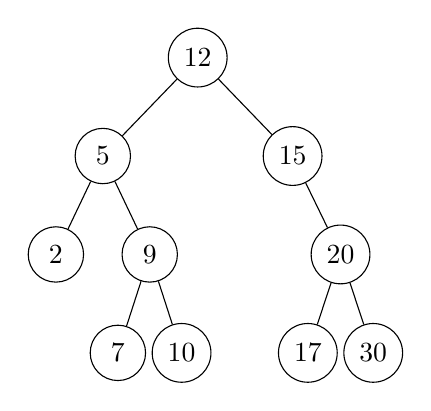
\begin{tikzpicture}
    \Tree
    [.12
    [.5
    2
        [.9
            7
            10
        ]
    ]
    [.15
    \edge[blank]; \node[blank]{};
    [.20
    17
    30
    ]
    ]
    ]
\end{tikzpicture}

\Q How would you delete 7?
\begin{answer}[1in]
\end{answer}

\Q How would you delete 15?
\begin{answer}[1in]
\end{answer}

\Q How would you delete 5?
\begin{answer}[1in]
\end{answer}

\newpage
In general, here is the strategy for deletion:
\par\vskip 10pt

\textbf{Delete(D, T):}

If Find(D, T) is false, do nothing.

If T is a leaf node, delete it and update its parent to point to null instead of T.

If T is an interior node and T has just a right child, delete T and update its parent to point to T's right child.

If T is an interior node and T has just a left child, delete T and update its parent to point to T's left child.

Else (T is interior with 2 children):
\par\vskip 10pt

Find the next successor of T by traversing to T's right child and then going all the way to the leftmost leaf.
This leftmost leaf is the next largest item in the tree.
Copy the value of this leftmost leaf to T.
If leftmost leaf does not have a right subtree, delete leftmost leaf with same procedure as leaf node above.
If leftmost leaf has a right subtree, then delete with the same procedure as interior node with just a right child.

\Q Delete node 5 with procedure above. Cross out nodes that are deleted and values that are updated.

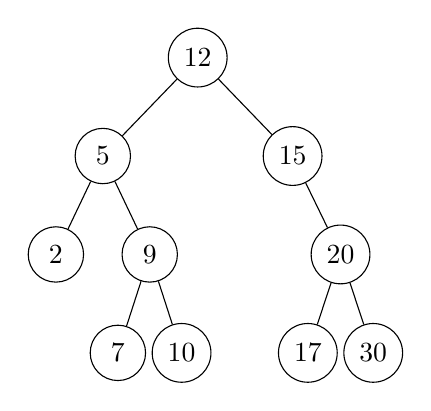
\begin{tikzpicture}
    \Tree
    [.12
    [.5
    2
        [.9
            7
            10
        ]
    ]
    [.15
    \edge[blank]; \node[blank]{};
    [.20
    17
    30
    ]
    ]
    ]
\end{tikzpicture}

\Q Delete node 10 with procedure above.
Cross out nodes that are deleted and values that are updated.

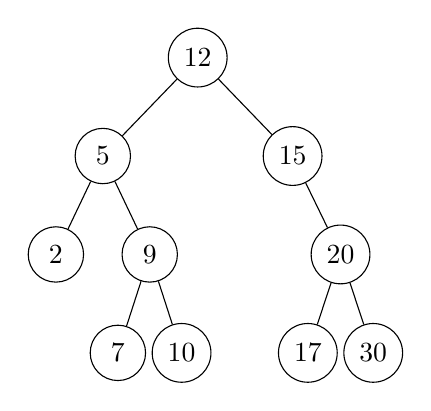
\begin{tikzpicture}
    \Tree
    [.12
    [.5
    2
        [.9
            7
            10
        ]
    ]
    [.15
    \edge[blank]; \node[blank]{};
    [.20
    17
    30
    ]
    ]
    ]
\end{tikzpicture}

\newpage
\Q Delete node 15 with procedure above.
Cross out nodes that are deleted and values that are updated.

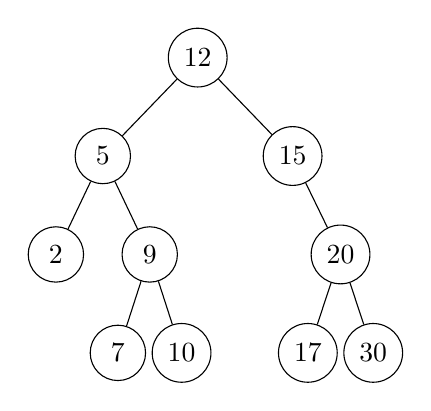
\begin{tikzpicture}
    \Tree
    [.12
    [.5
    2
        [.9
            7
            10
        ]
    ]
    [.15
    \edge[blank]; \node[blank]{};
    [.20
    17
    30
    ]
    ]
    ]
\end{tikzpicture}

Even though we are modeling BSTs with nodes having just one value, a (key, value) pair could be stored at each node, with the keys used as the comparison values when inserting, finding, and deleting.

\Q Does your group have any questions about binary search trees? Post them to teams under the \textit{Questions} channel.



\end{document}
